\chapter{Search Algorithm}

\href{https://www.youtube.com/watch?v=UXW2yZndl7U}{Reference: John Levine}

\section{Monte Carlo Tree Search}
Monte Carlo Tree Search (MCTS) is a search technique in the field of Artificial Intelligence (AI). It is a probabilistic and heuristic driven search algorithm that combines the classic tree search implementations alongside machine learning principles of reinforcement learning.

It consists of four phases:
\begin{itemize}
	\item Tree traversal
	\item Node expansion
	\item Rollout
	\item Backpropagation
\end{itemize}

In tree search, there's always the possibility that the current best action is actually not the most optimal action. In such cases, MCTS algorithm becomes useful as it continues to evaluate other alternatives periodically during the learning phase by executing them, instead of the current perceived optimal strategy. This is known as the ``exploration-exploitation trade-off''. It exploits the actions and strategies that is found to be the best till now but also must continue to explore the local space of alternative decisions and find out if they could replace the current best.

Exploration helps in exploring and discovering the unexplored parts of the tree, which could result in finding a more optimal path. In other words, we can say that exploration expands the tree's breadth more than its depth. Exploration can be useful to ensure that MCTS is not overlooking any potentially better paths. But it quickly becomes inefficient in situations with large number of steps or repetitions. In order to avoid that, it is balanced out by exploitation. Exploitation sticks to a single path that has the greatest estimated value. This is a greedy approach and this will extend the tree's depth more than its breadth. In simple words, UCB formula applied to trees helps to balance the exploration-exploitation trade-off by periodically exploring relatively unexplored nodes of the tree and discovering potentially more optimal paths than the one it is currently exploiting.

For this characteristic, MCTS becomes particularly useful in making optimal decisions in Artificial Intelligence (AI) problems.

\subsection{Tree Traversal}
In this process, the MCTS algorithm traverses the current tree from the root node using a specific strategy. The strategy uses an evaluation function to optimally select nodes with the highest estimated value. MCTS uses the Upper Confidence Bound (UCB) formula applied to trees as the strategy in the selection process to traverse the tree. It balances the exploration-exploitation trade-off. During tree traversal, a node is selected based on some parameters that return the maximum value. The parameters are characterized by the formula that is typically used for this purpose is given below:
$$\textrm{UCB1}(S_i) = \underbrace{\bar{V}_i}_{Exploitation} + \underbrace{C \sqrt{\frac{\ln N}{n_i}}}_{Exploration}, $$
\begin{itemize}
	\item $C$ is a balancing factor between exploitation and exploration.
	\item $N$ the number of visit of parent node
	\item $n_k$ the number of visit of node $k$
\end{itemize}
Let's say there are two successor nodes. One is visited more times than another one. Then, it means it is exploited more times than the other one. Thus, exploration term of the less exploited one would be higher than the highly visited one. By computing the UCB1 socre, the agent chooses a successor node with higher UCB1 score.
\subsection{Expanasion}
Expand successor node
\subsection{Rollout (Random Simulation)}
Simulation is completely random. In other words, we don't know how an agent reacts to an environment, so each successor state, the agent randomly decides which action to do till the termination. 
\subsection{Backpropagation}
Backpropagate rewards (value), and the number of visit at a node. 
\begin{itemize}
	\item $t$: total score
	\item $n_k := n_k+1$
\end{itemize}

\begin{figure}[h]
	\centering
	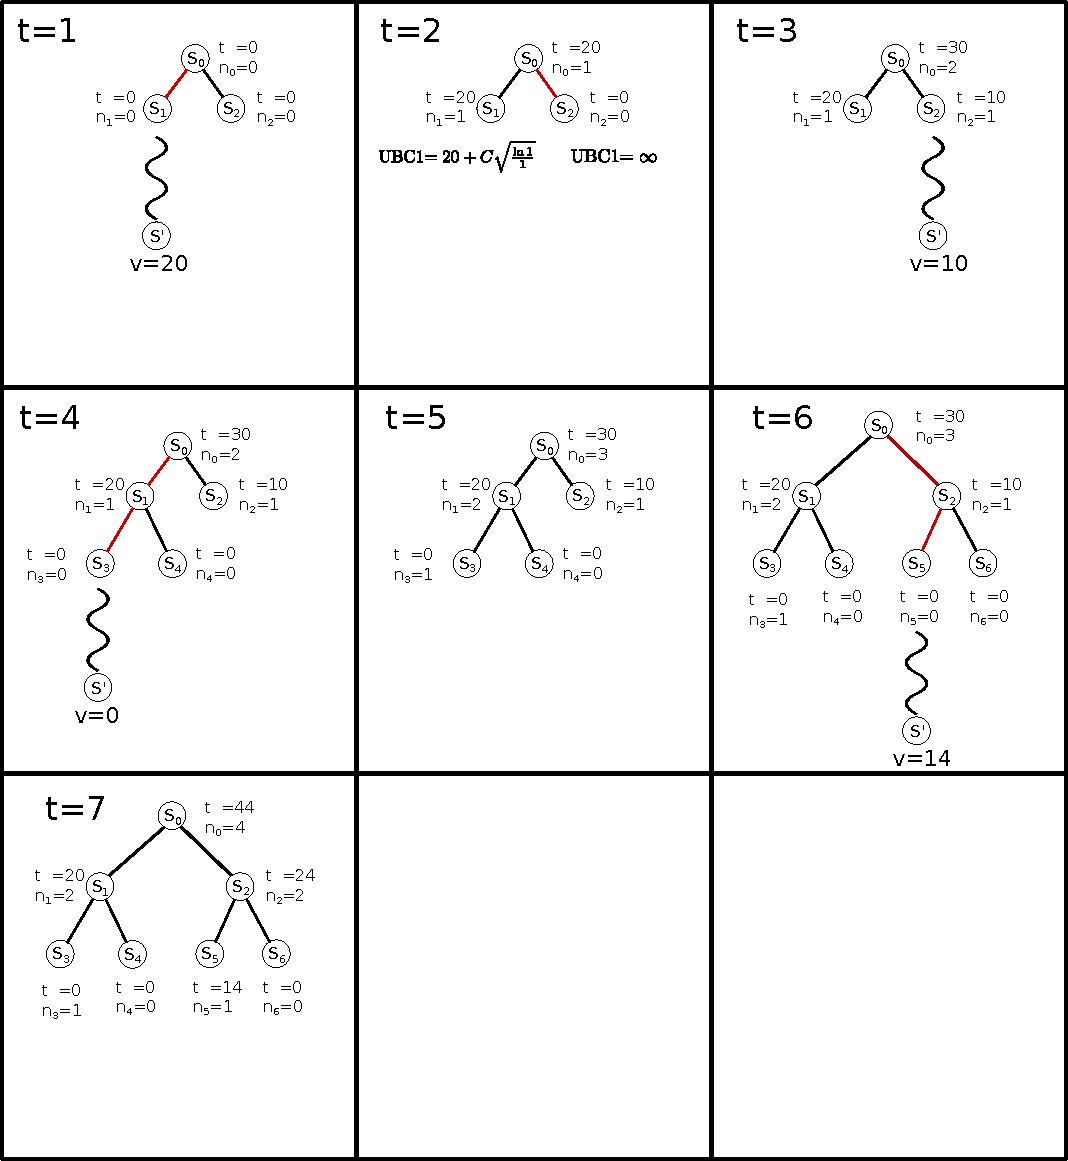
\includegraphics[scale=0.8]{./images/search_alg/mcts.pdf}
	\caption{MCTS example}
	\label{fig:mcts}
\end{figure}


\section{Uniform Cost Search}

You have three goal states, $G_1, G_2$, $G_3$. Your goal is to reach one of them. UCS is cheapest first search algorithm.

\begin{figure}[h]
	\centering
	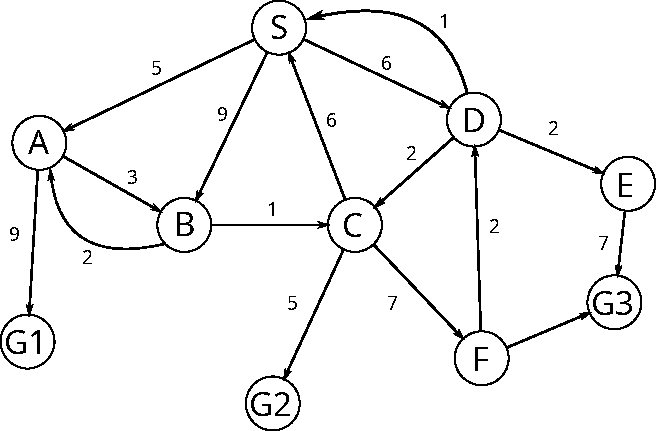
\includegraphics[scale=0.8]{./images/search_alg/uniform_sample_graph.pdf}
\end{figure}

\begin{figure}[h]
	\centering
	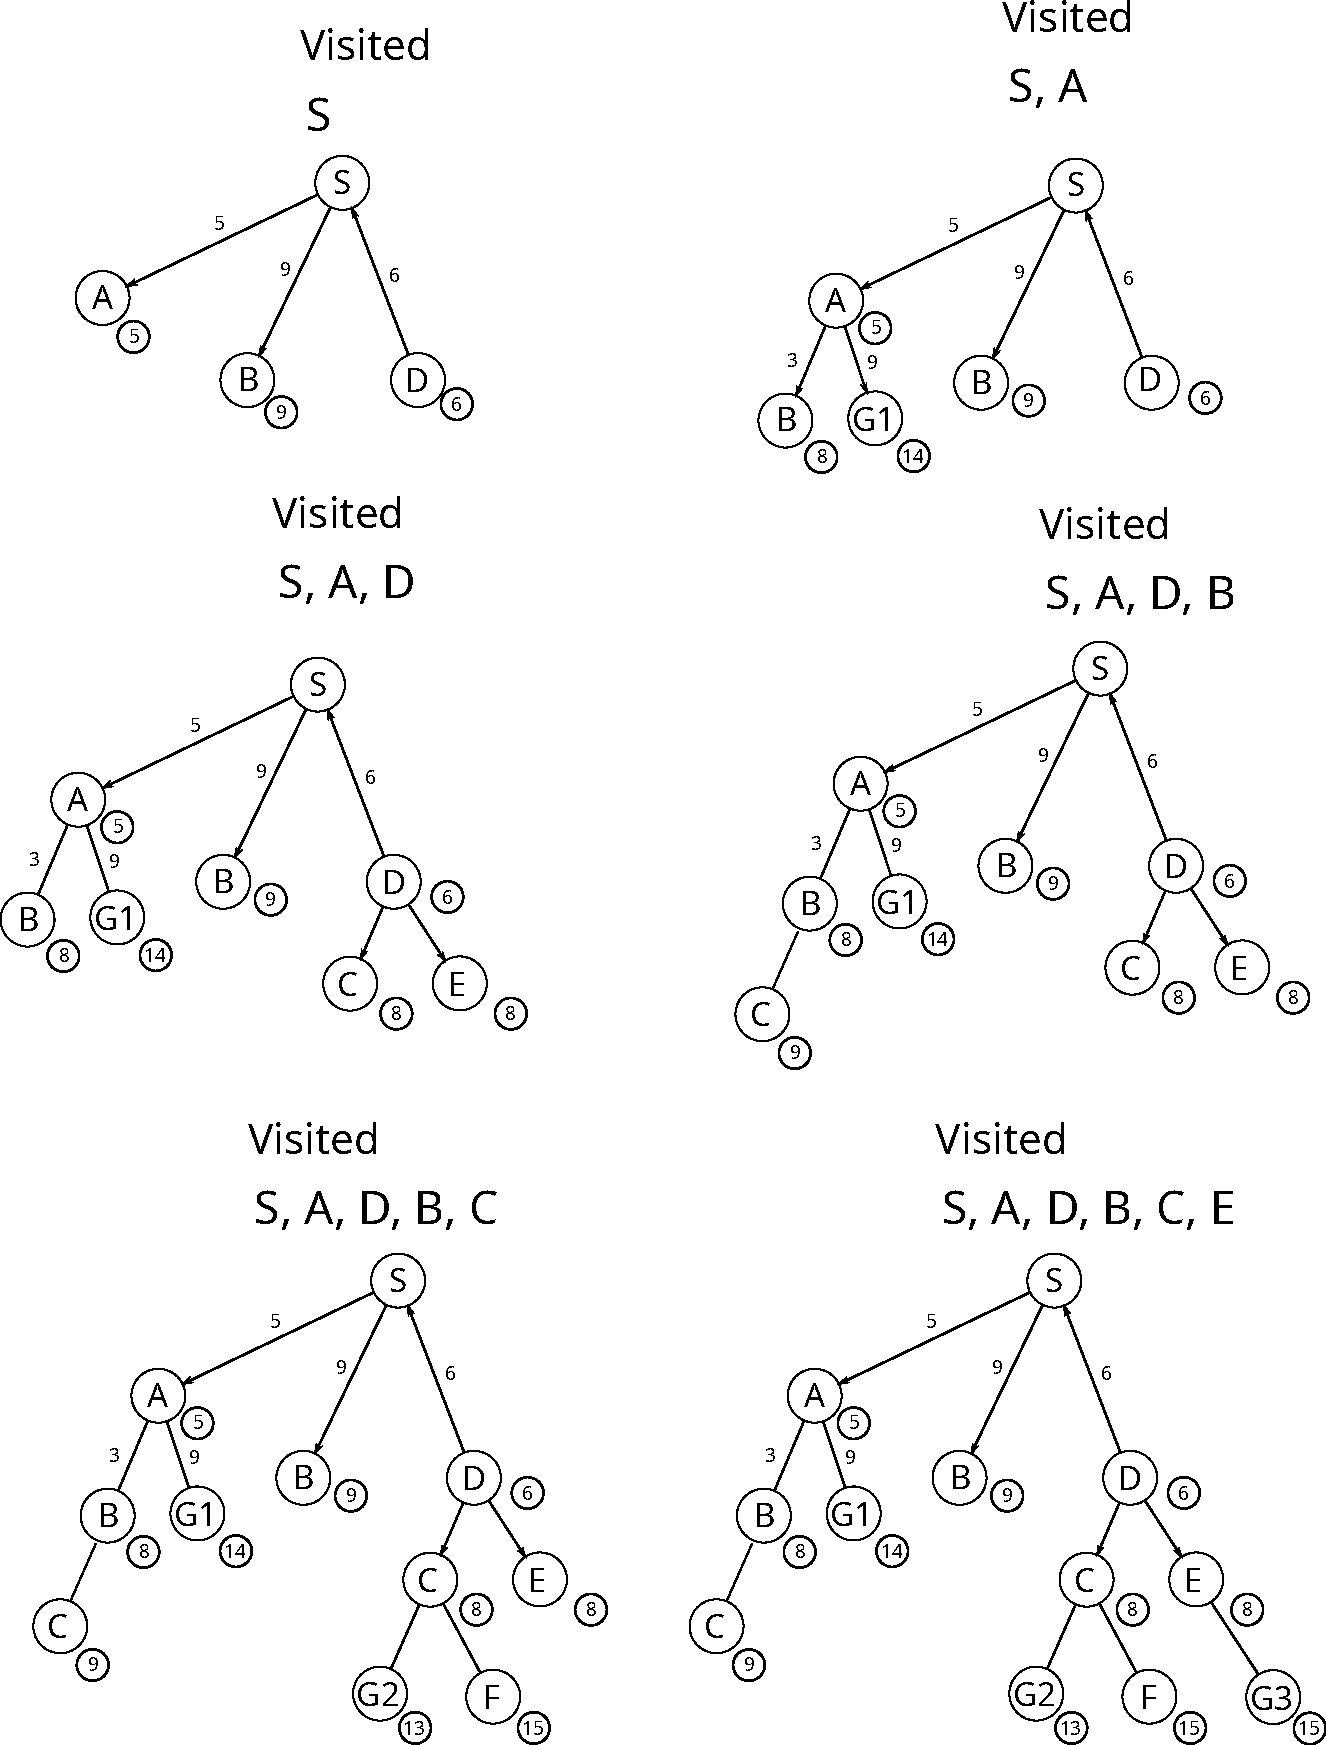
\includegraphics[scale=0.6]{./images/search_alg/uniform_cost_search.pdf}
\end{figure}

\newpage
\section{$A^*$ Search}
$A^*$ search algorithms is a variant of Dijkstra's algorithm, which incorporate additional \textit{heuristic} information about a graph. Unlike the Dijkstra's algorithm, you can specify a target node that you are interested in so that you don't have to compute all paths. 

In addition, the $A^*$ algorithm is often preferred over Dijkstra's algorithm in scenarios where the cost of reaching a goal from a particular node is not only determined by the actual distance traveled but also influenced by a heuristic estimation of the remaining distance to the goal. 

As I said, it exploits heuristics (or estimates). For instance, if we want to get a shortest path to a certain location in a map, then a very reasonable choice is to measure a distance roughly by using Euclidean distance. In \Cref{fig:astar_start}, we first initialize each node in the graph with our estimates. 

\begin{figure}[h]
	\centering
	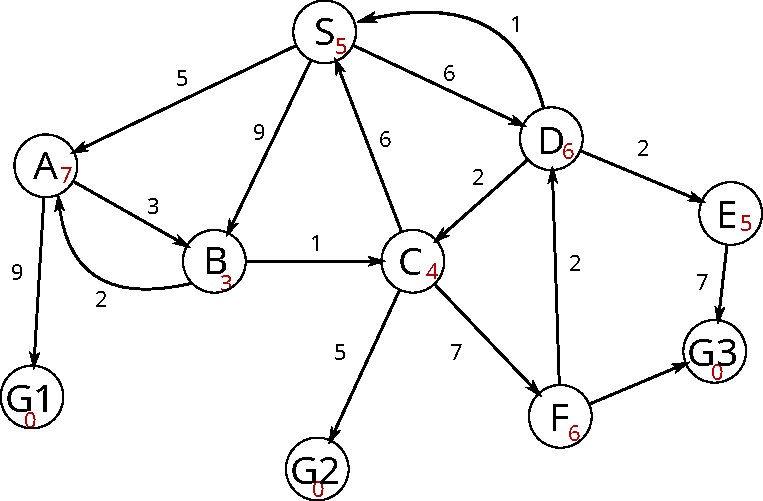
\includegraphics[scale=0.73]{./images/search_alg/astar_prob.pdf}
	\caption{Initialize $A^*$ search algorithm with heuristics.}
	\label{fig:astar_start}
\end{figure}

Then, we can explore as shown in \Cref{fig:astar_search}. For each visit, take a shortest path. 

\begin{figure}[h]
	\centering
	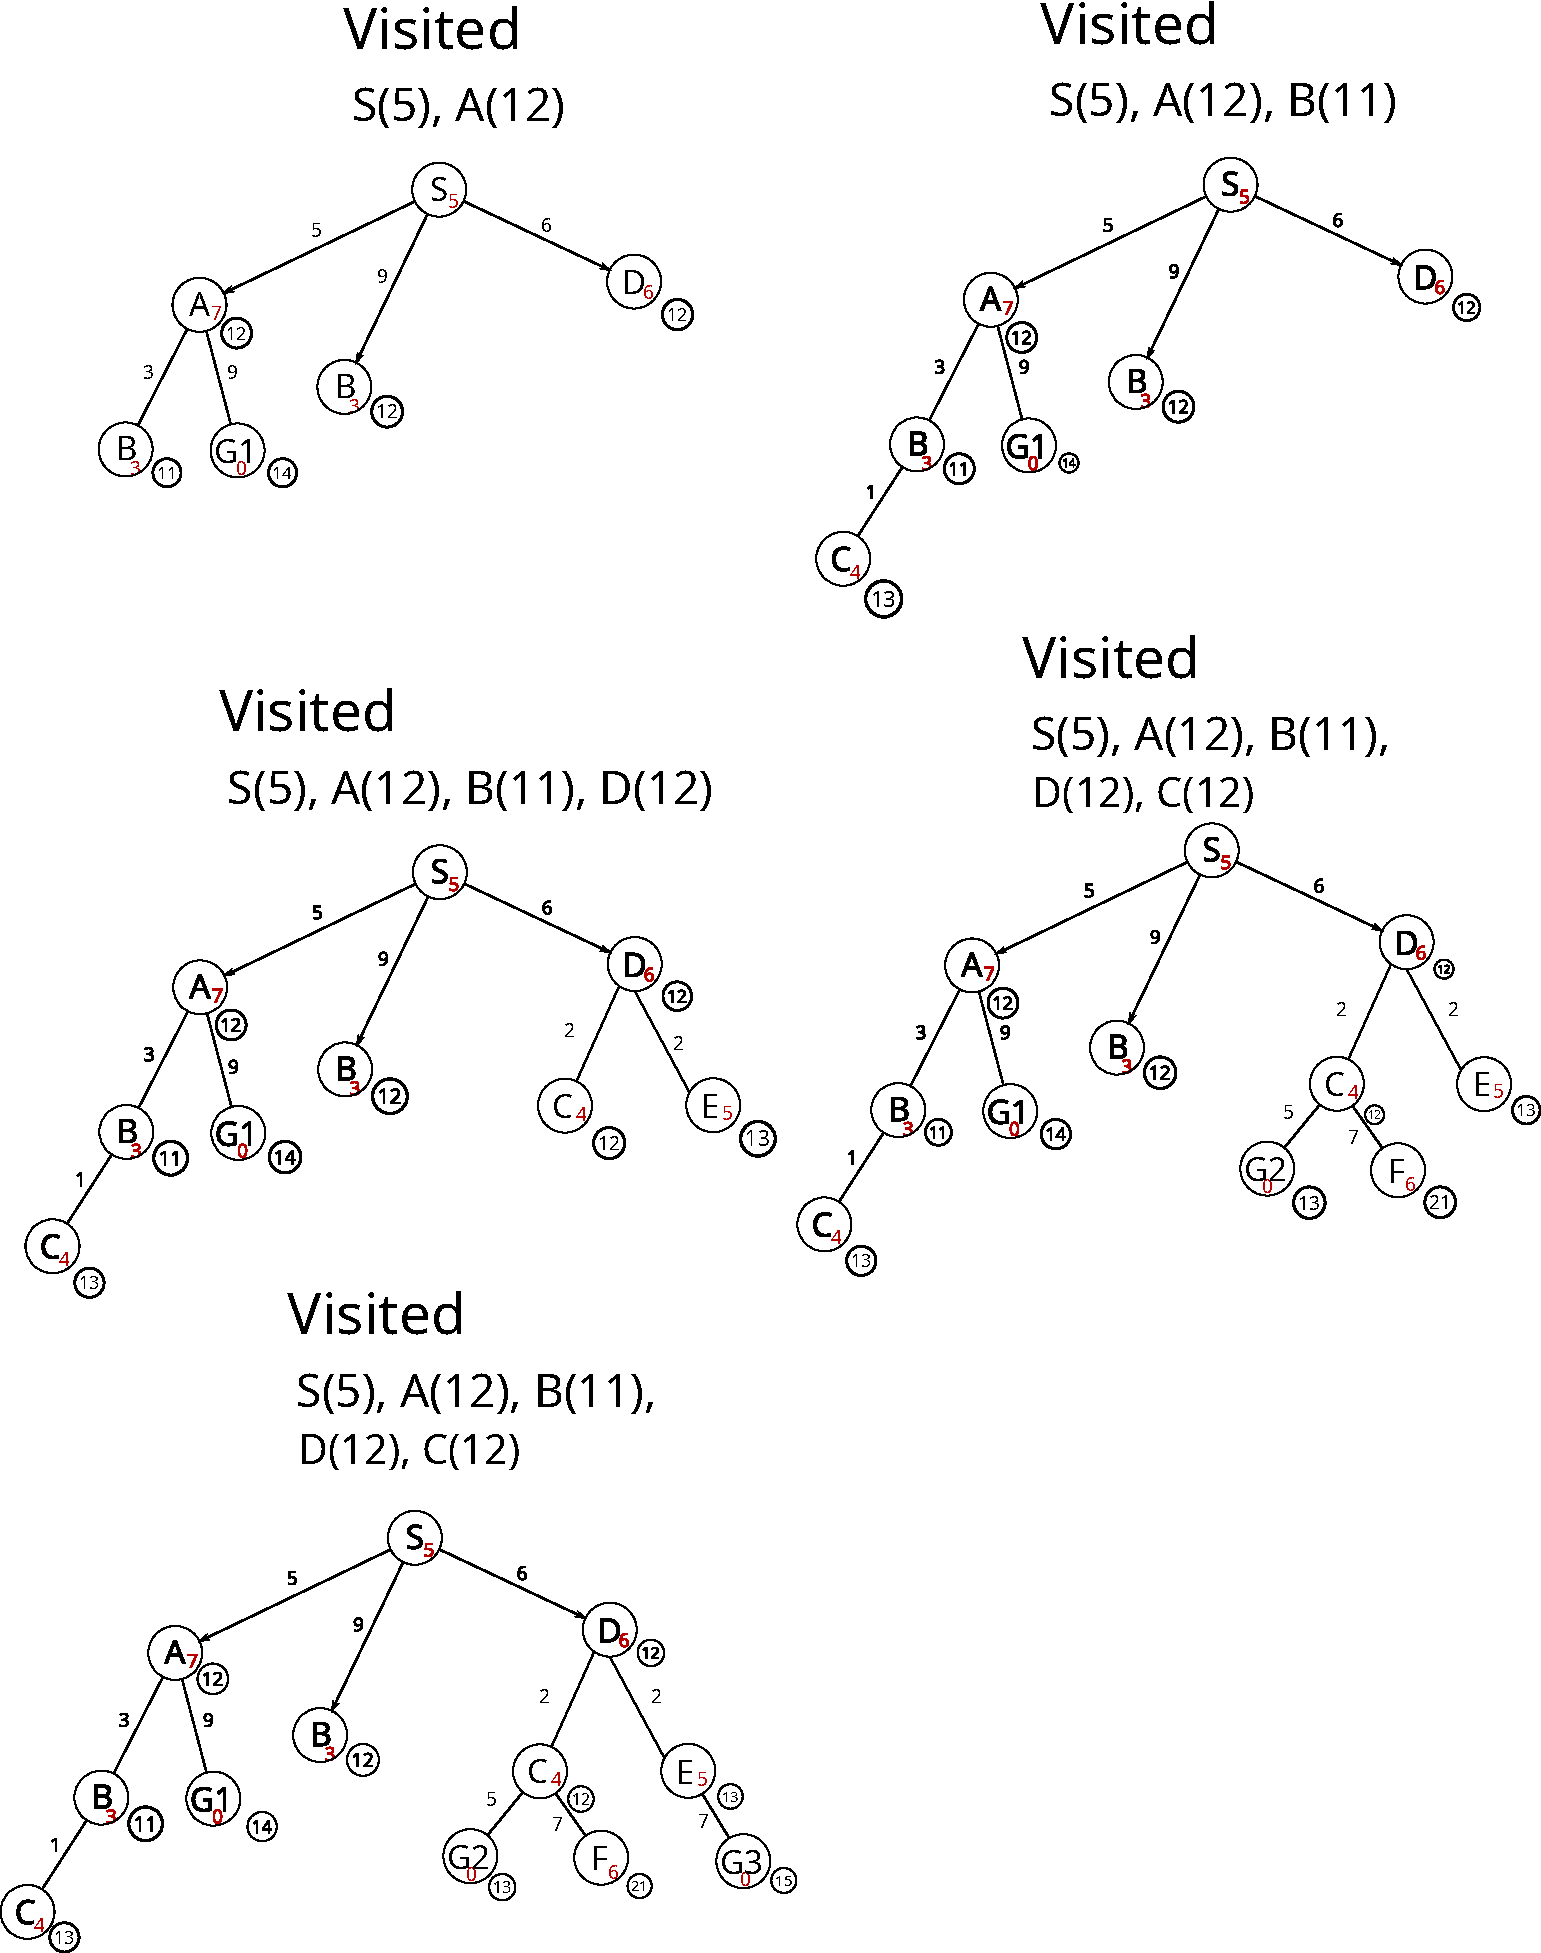
\includegraphics[scale=0.60]{./images/search_alg/astar_search.pdf}
	\label{fig:astar_search}
\end{figure}

Each number next to the nodes is called $A^*$ score, which is an estimate of cost to get to one of states. 

Note that $A^*$ algorithm is typically explained with open set and closed sets, which are just sets for nodes to be evaluated and visited. 

Open Set and Closed Set:
\begin{itemize}
	\item Open set contains nodes that need to be evaluated, 
	\item Closed set contains nodes that have already been evaluated.
\end{itemize}
